\documentclass[../main.tex]{subfiles}
\graphicspath{{\subfix{images/}}}

\begin{document}

\section{Results}



\subsection{The recommended content}

\begin{figure}[ht]
  \textbf{Conspiracy recommendations}\par\medskip
  \centering
  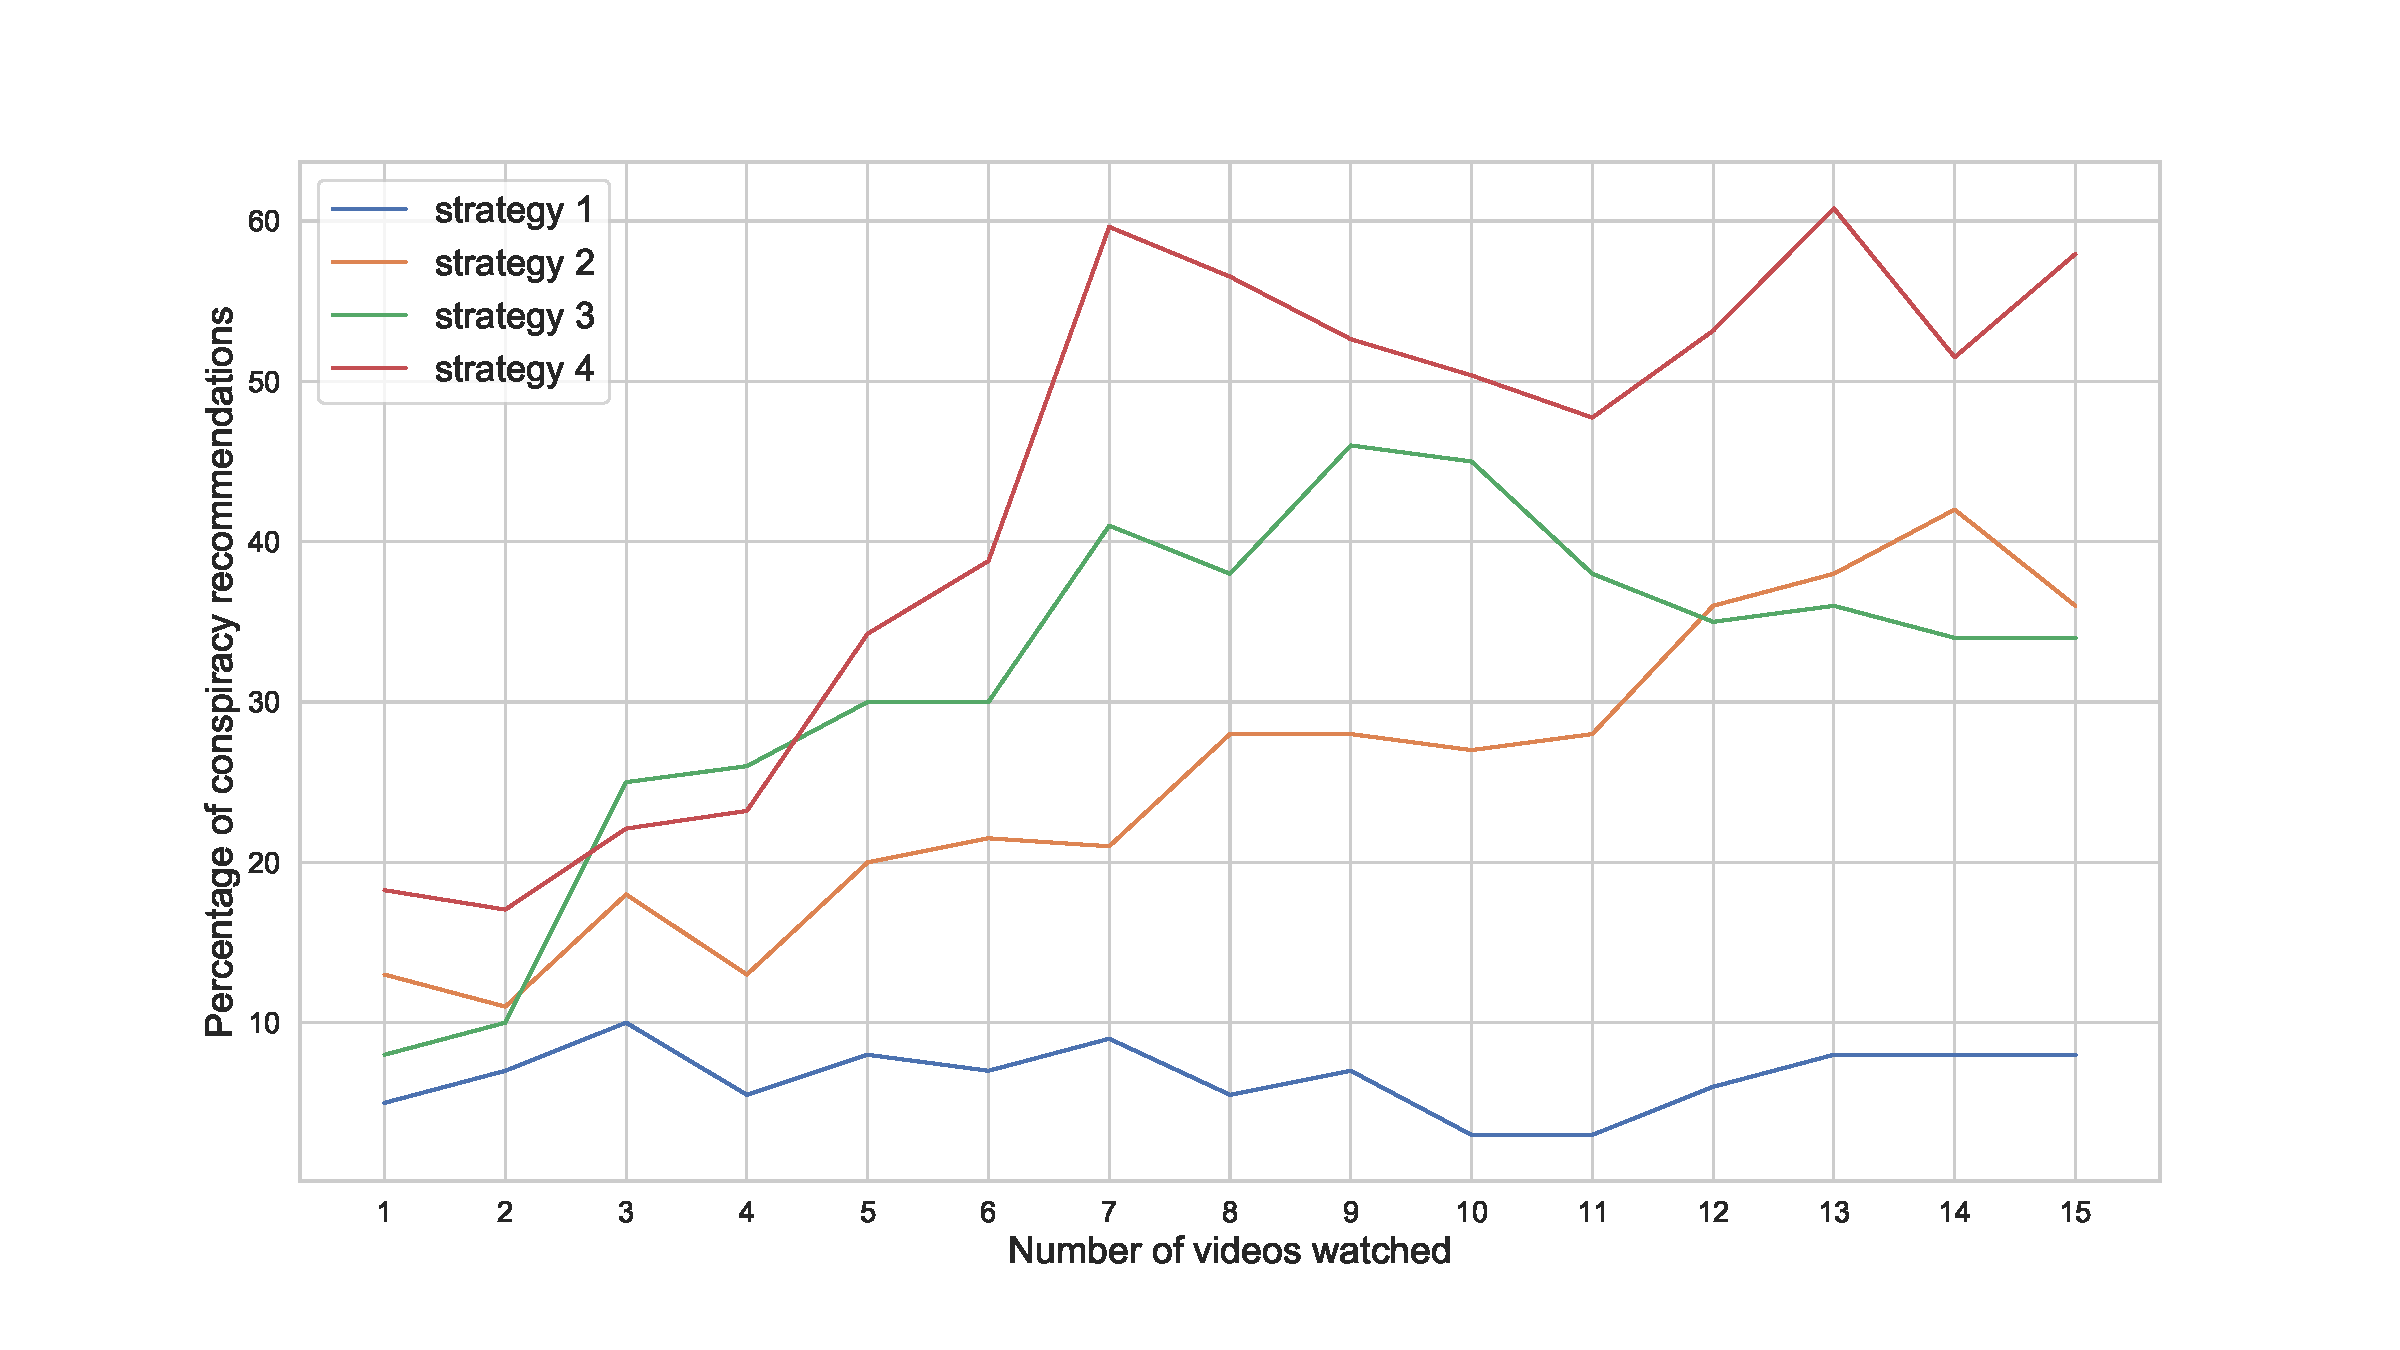
\includegraphics[keepaspectratio, width=\textwidth]{images/conspiracy_recs.pdf}
  \caption{The percentage of conspiracy recommendations after each number of videos per strategy}
  \label{fig:con_recs}
\end{figure}

\begin{itemize}
    \item All strategies except for the baseline lead to filter bubbles;
    \begin{itemize}
        \item strategy 4 had the biggest bubble;
        \item strategy 2 and 3 do not differ all too much, which is interesting;
        \item seems like YouTube sort of 'caps' the amount of conspiracy videos on the homepage, as each time a new height is reached, the number starts decreasing;
    \end{itemize}
    \item All strategies except the baseline lead to a lower diversity of content;
    \item Average views drop rapidly when a user starts watching content, regardless of the strategy;
    \begin{itemize}
        \item typical example of a cold-start problem;
    \end{itemize}
    \item The average duration of videos is higher for the conspiracy strategies, but it seems somewhat random.
    
\end{itemize}

\subsection{Leaving the filter bubble}

\begin{itemize}
    \item The number of conspiracy recommendations drops quickly, but keeps hovering a fair amount above baseline;
    \begin{itemize}
        \item This means that YouTube quickly adapts to the new content being watched, but still keeps the previous content in mind;
        \item The amount at which it hovers, seems to be proportional to the initial value of the filter bubble: if a user gets recommended more conspiracy content at first, more of that will stay once they stop watching that type of content; 
    \end{itemize}
    \item The number of videos until the algorithm stops recommending conspiracy content is well over 15;
    \item This is interesting, as a user ends up in a bubble after $\pm 5$ videos watched.
\end{itemize}

\subsection{Machine learning}

\begin{figure}[t!]
  \textbf{Classifier performance}\par\medskip
  \centering
  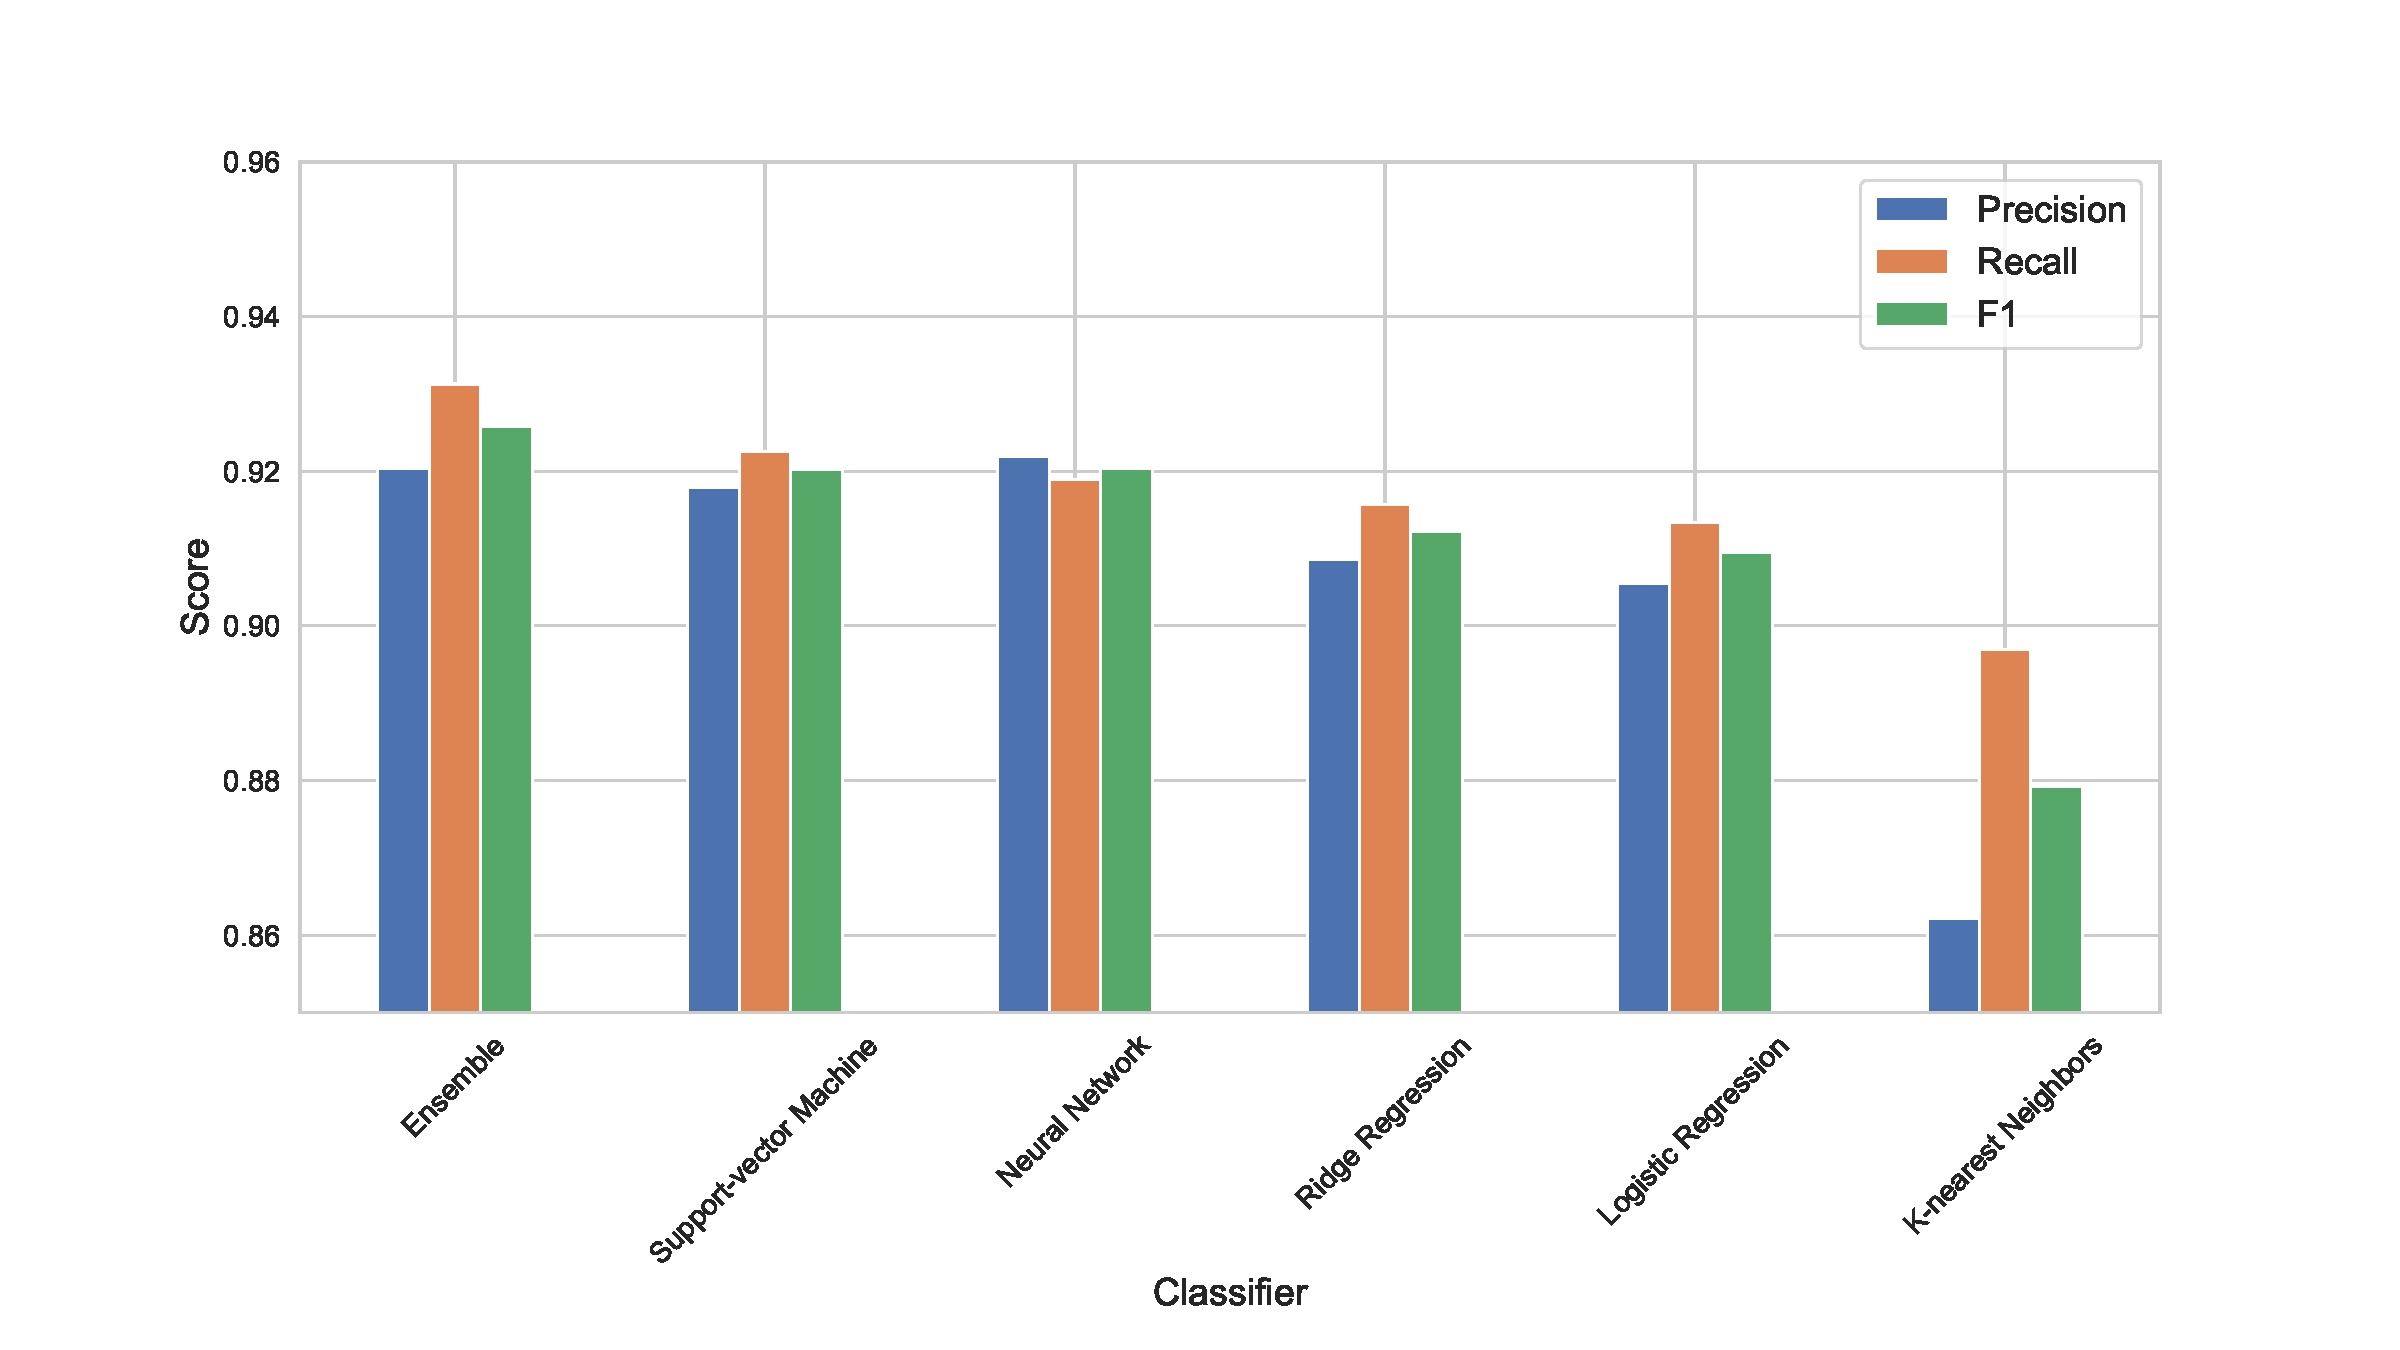
\includegraphics[keepaspectratio, width=\textwidth]{images/classifier_results.pdf}
  \caption{Metrics for each classifier with optimized hyperparameters}
  \label{fig:ML_scores}
\end{figure}

The hyperparameter tuning lead to impressive scores for all classifiers. When making predictions for the
test set, the best-performing classifier is the support-vector machine making use of the Radial Basis
Function (RBF) kernel and a penalty parameter (C-value) of 10. The SVM is tied for F1-score with the neural 
network using the identity activation function, with 10 hidden layers of 10 neurons. Ridge regression with a 
sparse-cg solver and penalty (alpha) value of 0.1 takes the third place, very closely followed by logistic 
regression with an L2 penalty, a penalty (C) value of 20 and a newton-cg solver. The worst-performing 
classifier is also the simplest of the bunch: the k-nearest neighbors classifier (K=1). Although its 
performance is still formidable, it does substantially worse than the others. An overview of all metrics for 
each classifier can be seen in figure \ref{fig:ML_scores}. The ten best-performing configurations for each
classifier can be found in appendix \ref{appendix:Hyperparameters}.

Noteworthy is the fact that the optimal ensemble actually outperforms the support-vector machine by a
slight margin. This ensemble, consisting of the SVM, the neural network, and surprisingly, the k-nearest
neighbor classifiers, gets slightly higher scores than the runner-up across the board. The ensemble had
a 16-way tie for best-performing parameters, all of which contained at least the SVM, neural network,
and k-NN classifiers. 

Though the ensemble outperforms the other classifiers, it has a significant drawback: its training time
is significantly larger than that of the individual classifiers. Support-vector machines are infamous
for their slowness when there is a lot of training data, and neural networks can require a lot of
training time whenever the number of neurons gets large \citep{burges1997improving,
kamarthi1999accelerating}. Requiring both algorithms to run will therefore require a lot of additional
training time. Considering the marginal performance increase, the cost outweighs the benefit. As a
result, when taking everything into account, the support-vector machine is the best classifier for
labeling conspiracy videos on YouTube.

Additionally, for predicting the likelihood of recommendations being conspiracy videos in real-time, as was 
done for strategy 3 and 4, the best-performing classifier is the neural network. Here, the neural network is
preferred over the support-vector machine, as neural networks are better optimized for providing 
probabilities of samples belonging to a certain class \citep{specht1990probabilistic}.
\end{document}